\subsection{\textsc{K-Dist} algorithm}

This section presents the \textsc{K-Dist} algorithm used in \texttt{klust}.
\textsc{K-Dist} uses a window of length equal to the shortest of the two
sequences being compared. The distance between the substrings in the initial,
leftmost position of the window is calculated using a variant of the basic
\textsc{d2} algorithm. The window then iterates over the longer sequence, one
nucleotide at a time, and calculates the new distance between the substring of
the longer sequence and the shorter sequence.  This calculation is done using a
kind of forward differences method for reducing the calculations to a few fixed
operations for calculating the distance in the next window from the distance in
the current window. S. Hazelhurst~\cite{hazelhurst} describes this concept and
uses it in a variant of the \textsc{d2} algorithm.

\textsc{K-Dist} uses the \emph{Manhattan distance}~\cite{upton} instead of the
Euclidean distance used in the \textsc{d2} algorithm for calculating the
distance between the two $k$-mer frequency vectors. The Manhattan distance is
similar to the Euclidean distance but with squaring replaced with absolute
value and the square root omitted, i.e.  for $u, v \in \mathbb{Z}^n$,

\begin{equation*}
  d_{Manhattan} \eqdef \sum_{i=1}^{n} |u_i - v_i| \;.
\end{equation*}

This distance metric was chosen for simplicity, to make the calculation of
distance in subsequent window positions easier, which also improves
performance, and since there is evidence in the literature that the Manhattan
distance generally is preferable to Euclidean distance for high dimensional
distance calculation~\cite{aggarwal}.

To calculate the distance in the next window position from the distance in the
current window, i.e. advancing the window through the longer of the two
sequences by one character, it is decided which $k$-mers exit and enter the
window, respectively, and then by looking at whether the existing $k$-mer count
in the frequency vector is negative or positive, it can be decided whether the
distance increases or decreases by 2 or if it stays the same.
Subsequently, the frequency vector is updated to reflect the change in the new
window. Figure \ref{fig:d2_forward_differences} illustrates the idea of a
window and $k$-mers exiting and entering the window:

\begin{figure}[H]
\centering
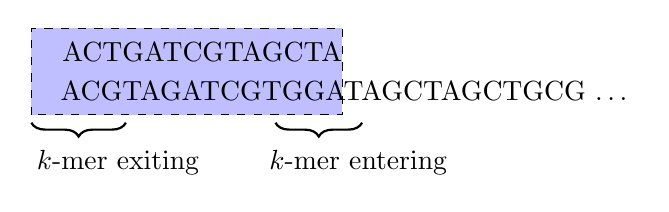
\begin{tikzpicture}
  \draw [fill=blue!25,dashed] (0,0.7) rectangle (3.95,1.8);
  \node at (4.0,1.5) {ACTGATCGTAGCTA\phantom{TAGCTAGCTGCG \dots}};
  \node at (4.0,1.0) {ACGTAGATCGTGGATAGCTAGCTGCG \dots};
  \draw [thick,decorate,decoration={brace,amplitude=5pt,mirror}]
    (0.0,0.6) -- (1.2,0.6) node[midway,xshift=0.5cm,yshift=-0.5cm]
    {$k$-mer exiting};
  \draw [thick,decorate,decoration={brace,amplitude=5pt,mirror}]
    (3.1,0.6) -- (4.2,0.6) node[midway,xshift=0.5cm,yshift=-0.5cm]
    {$k$-mer entering};
\end{tikzpicture}
\caption{Illustration of $k$-mers, where $k=4$, entering and exiting a window.}
\label{fig:d2_forward_differences}
\end{figure}

A distance measure, i.e. not a relative similarity measure, can be difficult to
use directly for determining sequence similarity, since the distance metric is
very dependent on the length of the shortest sequence (the length of the
window). For this reason, the ratio between the Manhattan distance and the
maximum possible distance in the window is used to normalize the distance to a
value in the interval $[0,1]$. Let $w$ denote the size of the window. The
corresponding similarity measure for the Manhattan distance in the window is
given by the following expression:

\begin{equation}
  1 - \frac{d_{Manhattan}(s,t)}{2(w - k + 1)} \label{eq:Manhattan_similarity}
\end{equation}

An alternative notion of similarity, which was the inspiration for the above
similarity measure, is the \emph{Jaccard index}~\cite{jaccard1912}, which is
defined as the size of the intersection of two sets divided by the size of the
union of the sets.  However, the Jaccard index does not take the multiplicity
of the elements into account and therefore it might give a lower sensitivity
than the similarity measure in equation (\ref{eq:Manhattan_similarity}).

The \textsc{K-Dist} algorithm (Algorithm \ref{alg:K-Dist}) has been implemented
and is used as the distance metric in the \texttt{klust} program.  The update
$cur\_dist$, $\mathtt{kmers}[x]$ and $\mathtt{kmers}[y]$ statement looks at the
values for specific $k$-mers $x$ and $y$ in the $k$-mer vector, increments or
decrements the values and updates the $cur\_dist$ accordingly.

\begin{algorithm}[H]
  \caption{\textsc{K-Dist} algorithm}
  \label{alg:K-Dist}
  \begin{algorithmic}[1]
    \Require{$s$ and $t$ are DNA or RNA sequences, $k \in \mathbb{Z}^+$}
    \Statex
    \Function{K-Dist}{$s, t, k$}
      \State set $s$ to the shorter sequence and $t$ to the longer sequence
      \State initialize map \texttt{kmers} : \texttt{string} $\to$
        \texttt{int} (0 initialized on first access)
      \State $cur\_dist \gets 0$
      \State
      \For{$i \gets 0$ to $\abs{s} - k$}
        \Comment{\parbox[t]{.3\linewidth}{$k$-mer counting}}
        \State $s_i \gets s.substring(i, k)$
        \State $t_i \gets t.substring(i, k)$
        \State update $cur\_dist$, $\mathtt{kmers}[s_i]$ and $\mathtt{kmers}[t_i]$
      \EndFor
      \State
      \State $min\_dist \gets cur\_dist$
      \For{$i \gets 0$ to $\abs{t} - \abs{s}$}
          \Comment{\parbox[t]{.3\linewidth}{No. of windows}}
        \State $kmer_{out} \gets t.substring(i, k)$
        \State $kmer_{in} \gets t.substring(\abs{s}-k+i+1, k)$
        \State update $cur\_dist$, $\mathtt{kmers}[kmer_{out}]$
               and $\mathtt{kmers}[kmer_{in}]$
        \State $min\_dist \gets min(min\_dist, cur\_dist)$
      \EndFor
      \State
      \State $max\_dist \gets 2\left(\abs{s}-k+1\right)$
      \State \Return{$(max\_dist-min\_dist) / max\_dist$}
    \EndFunction
  \end{algorithmic}
\end{algorithm}


\subsubsection{Complexity analysis} \label{sec:k-dist_analysis}

The \textsc{K-Dist} algorithm consists of two loops and a number of constant
time operations outside of the loops. In the first loop, the \textsc{K-Dist}
algorithm iterates over the first $|s|-k$ characters, where $|s|$ denotes the
length of the shorter of the two sequences. Each iteration contains only
constant time operations. This gives a running time of $\Theta(\abs{s}-k)$ since
the number of iterations is bounded both from below and from above by
$\abs{s}-k$. This is assuming that the map lookup is $\mathcal{O}(1)$ and that
the $substring$ method is constant time as well, which is the case when
strings are implemented as character arrays, assuming no copying is needed.

In the second loop, \textsc{K-Dist} performs $|t|-|s|$ iterations which each
contains a constant number of constant time operations. This gives a running
time of $\Theta(\abs{t}-\abs{s})$. This yields a total running time of:
\begin{align*}
  \Theta(\abs{s}-k) + \Theta(\abs{t}-\abs{s})
  &= \Theta(\abs{s} - k + \abs{t} - \abs{s}) \\
  &= \Theta(\abs{t} - k) \;.
\end{align*}

More generally, given two string $s$ and $t$ and $k \in \mathbb{Z}^{+}$, the
\textsc{K-Dist} algorithm has a worst case, average case and best case running
time of $\Theta(\max{\left(\abs{s}, \abs{t}\right)} - k)$.

The space usage of \textsc{K-Dist} depends on the value of $k$ and the $k$-mers
occurring in the sequences, since this affects the size of the \texttt{kmers}
map. The worst case space complexity is $\mathcal{O}\left(4^k\right)$, i.e.
exponential in the value of $k$, however, since $k$ is generally assumed
to be less than or equal to 8, the space usage should not become a problem.
